% Begin the document and set up the style of the document
\documentclass[a4paper]{article}

% Install the required packages for the document 
\usepackage{envmath}
\usepackage{esvect}
\usepackage{graphicx}
\usepackage{gensymb}
\usepackage{tikz}
\usepackage{geometry}
\usepackage{enumitem}
\usepackage{mathtools}
\usepackage{graphicx}
\usepackage{amsmath}
\usepackage{amscd}
\usepackage{amssymb}
\usepackage{amsfonts}
\usepackage{pgf}
\usepackage{tikz}
\usepackage{mathrsfs}
\usepackage{asyalign}
\usepackage{physics}
\usepackage{cite}
\usepackage{url}
\usepackage[tableposition=top]{caption}
\usepackage{ifthen}
\usepackage[utf8]{inputenc}
\usetikzlibrary{arrows}

\begin{document}

\begin{center}
	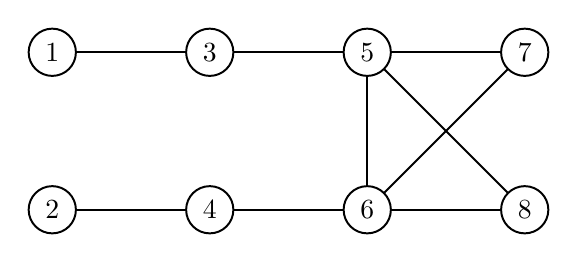
\begin{tikzpicture}

		\draw[line width = 0.25mm] (-3,2) circle (3mm);
		\node at (-3,2) {$1$};
		\draw[line width = 0.25mm] (-1,2) circle (3mm);
		\node at (-1,2) {$3$};
		\draw[line width = 0.25mm] (1,2) circle (3mm);
		\node at (1,2) {$5$};
		\draw[line width = 0.25mm] (3,2) circle (3mm);
		\node at (3,2) {$7$};

		\draw[line width = 0.25mm] (-3,0) circle (3mm);
		\node at (-3,0) {$2$};
		\draw[line width = 0.25mm] (-1,0) circle (3mm);
		\node at (-1,0) {$4$};
		\draw[line width = 0.25mm] (1,0) circle (3mm);
		\node at (1,0) {$6$};
		\draw[line width = 0.25mm] (3,0) circle (3mm);
		\node at (3,0) {$8$};

		\draw[line width = 0.25mm] (-2.70,2) -- (-1.3,2);
		\draw[line width = 0.25mm] (-0.70,2) -- (0.70,2);
		\draw[line width = 0.25mm] (1.3,2) -- (2.70,2);

		\draw[line width = 0.25mm] (-2.70,0) -- (-1.3,0);
		\draw[line width = 0.25mm] (-0.70,0) -- (0.70,0);
		\draw[line width = 0.25mm] (1.3,0) -- (2.70,0);

		\draw[line width = 0.25mm] (1.21,1.79) -- (2.79,0.21);
		\draw[line width = 0.25mm] (1.21,0.21) -- (2.79,1.79);
		\draw[line width = 0.25mm] (1,1.70) -- (1,0.30);

	\end{tikzpicture}
\end{center}

\end{document}